\documentclass[11pt]{article}\usepackage[]{graphicx}\usepackage[]{color}
% maxwidth is the original width if it is less than linewidth
% otherwise use linewidth (to make sure the graphics do not exceed the margin)
\makeatletter
\def\maxwidth{ %
  \ifdim\Gin@nat@width>\linewidth
    \linewidth
  \else
    \Gin@nat@width
  \fi
}
\makeatother

\definecolor{fgcolor}{rgb}{0.345, 0.345, 0.345}
\newcommand{\hlnum}[1]{\textcolor[rgb]{0.686,0.059,0.569}{#1}}%
\newcommand{\hlstr}[1]{\textcolor[rgb]{0.192,0.494,0.8}{#1}}%
\newcommand{\hlcom}[1]{\textcolor[rgb]{0.678,0.584,0.686}{\textit{#1}}}%
\newcommand{\hlopt}[1]{\textcolor[rgb]{0,0,0}{#1}}%
\newcommand{\hlstd}[1]{\textcolor[rgb]{0.345,0.345,0.345}{#1}}%
\newcommand{\hlkwa}[1]{\textcolor[rgb]{0.161,0.373,0.58}{\textbf{#1}}}%
\newcommand{\hlkwb}[1]{\textcolor[rgb]{0.69,0.353,0.396}{#1}}%
\newcommand{\hlkwc}[1]{\textcolor[rgb]{0.333,0.667,0.333}{#1}}%
\newcommand{\hlkwd}[1]{\textcolor[rgb]{0.737,0.353,0.396}{\textbf{#1}}}%
\let\hlipl\hlkwb

\usepackage{framed}
\makeatletter
\newenvironment{kframe}{%
 \def\at@end@of@kframe{}%
 \ifinner\ifhmode%
  \def\at@end@of@kframe{\end{minipage}}%
  \begin{minipage}{\columnwidth}%
 \fi\fi%
 \def\FrameCommand##1{\hskip\@totalleftmargin \hskip-\fboxsep
 \colorbox{shadecolor}{##1}\hskip-\fboxsep
     % There is no \\@totalrightmargin, so:
     \hskip-\linewidth \hskip-\@totalleftmargin \hskip\columnwidth}%
 \MakeFramed {\advance\hsize-\width
   \@totalleftmargin\z@ \linewidth\hsize
   \@setminipage}}%
 {\par\unskip\endMakeFramed%
 \at@end@of@kframe}
\makeatother

\definecolor{shadecolor}{rgb}{.97, .97, .97}
\definecolor{messagecolor}{rgb}{0, 0, 0}
\definecolor{warningcolor}{rgb}{1, 0, 1}
\definecolor{errorcolor}{rgb}{1, 0, 0}
\newenvironment{knitrout}{}{} % an empty environment to be redefined in TeX

\usepackage{alltt}
%Required: You must have these
\usepackage{graphicx}
\usepackage{tabularx}
\usepackage{natbib}
\usepackage{pdflscape}
\usepackage{array}
\usepackage{authblk}
\usepackage{gensymb}
\usepackage{amsmath}
%\usepackage[backend=bibtex]{biblatex}
\usepackage[small]{caption}

\setkeys{Gin}{width=0.8\textwidth}
\setlength{\captionmargin}{30pt}
\setlength{\abovecaptionskip}{10pt}
\setlength{\belowcaptionskip}{10pt}

 \topmargin -1.5cm 
 \oddsidemargin -0.04cm 
 \evensidemargin -0.04cm 
 \textwidth 16.59cm
 \textheight 21.94cm 
 \parskip 7.2pt 
\renewcommand{\baselinestretch}{1.6} 	
\parindent 0pt
\usepackage{setspace}
\usepackage{lineno}

\bibliographystyle{..//..//sub_projs/refs/styles/besjournals.bst}
\usepackage{xr-hyper}
\usepackage{hyperref}
\externaldocument{SUPP_FLS_flobud}

\linenumbers
\title{Differences in flower and leaf bud environmental responses drive shifts in spring phenological sequences of temperate woody plants}
\date{}
\author{D.M. Buonaiuto $^{1,2,a}$, E.M. Wolkovich$^{3}$}
\IfFileExists{upquote.sty}{\usepackage{upquote}}{}
\begin{document}
\maketitle
\noindent \emph{Author affiliations:}\\
\noindent $^1$Arnold Arboretum of Harvard University, Boston, Massachusetts, USA. ORCID: 0000-0003-4022-2591\\
$^2$Department of Organismic and Evolutionary Biology, Harvard University, Cambridge, Massachusetts, USA \\
$^3$Forest \& Conservation Sciences, Faculty of Forestry, University of British Columbia, Vancouver, British Columbia, Canada\\
$^a$Corresponding author: 617.823.0687; dbuonaiuto@g.harvard.edu\\

\textbf{Acknowledgements:} We thank C. de Keyzer for generously helping to collect and prepare plant materials for the experiment. We also thank R. Lee for help with monitoring and maintaining the experiment.\\

\textbf{Author Contributions:} DMB and EMW conceived of the experiment; DMB collected the data and performed the statistical analyses, DMB and EMW wrote the manuscript. All authors contributed critically to the drafts and gave final approval for publication.\\

\textbf{Data Availability Statement:} Data will be available on KNB upon publication. All modeling code will be made available upon request.

\pagebreak


\maketitle
\section*{Abstract} 
The relative timing of growth and reproduction is an important driver of plant fitness. For deciduous woody species in temperate regions leaves and flowers both appear in the early spring, but the order and duration of these phenological events vary among species, populations, and individuals. This observed variation in flower-leaf sequences (FLSs) suggests that the relative timing of these events may be important---affecting the reproduction, recruitment and survival of individuals. Further, FLSs appear to be shifting with climate change, and anticipating the extent of these shifts is key to projecting how climate change may impact species' performance and reshape forest communities. Predicting FLS shifts, however, requires an improved understanding of how the environment dictates FLS patterns. To address this, we compared the phenological responses of flower and leaf buds for 10 temperate woody species to varying levels of temperature and light in a lab experiment. Our experimental design allowed us to test competing hypotheses for how environmental cues determine FLS variation---specifically whether forcing (warm temperatures) alone drives variation or differential sensitivity to chilling (cool temperatures generally in the fall and winter) and/or photoperiod matter. We found that flower and leaf buds respond with differential sensitivity to environmental cues, with differences in their response to chilling being the dominant driver of FLS variation. Because climate change will amplify variability in chilling across time and space, these findings suggest that FLS shifts may be large, but are likely to vary substantially among populations and species. In our study, FLS shifts were largest in wind-pollinated species that flower before leafing, raising the possibility that, more generally, wind-pollinated taxa may experience reproductive declines due to FLS shifts in the decades to come.   \\ % 253 words out of 350 permitted

\noindent \emph{Keywords:} chilling, climate change, deciduous forests, differential sensitivity, flower-leaf sequences, forcing, hysteranthy, phenology  \\ 

\section*{Introduction}
\noindent Among the most widely documented biological effects of anthropogenic climate change are shifts in plant phenology, the timing of life cycle events \citep{Parmesan2003,Menzel2006,Cleland2007}. While phenology is generally advancing with climate change, the strength of these phenological shifts can vary substantially among specific phenological phases \citep{Augspurger:2020aa}. These differences alter the timing of phases relative to each other, changing the duration between events that make up phenological sequences \citep{Ettinger2018}. Phenological sequences are a major driver of plant fitness that impacts plant life history, resource allocation, demography and ecosystem processes \citep{Post:2008aa}. Thus, shifting sequences with climate change will likely impact many of these processes. The effects of these shifts, however, depend both on their direction---whether distinct phases are shifting closer together or farther apart---and magnitude---how much they are shifting relative to each other.\\ 

\noindent Among deciduous woody plants, the relative timing of flower and leaf phenology, or flower-leaf sequences (FLSs), may be particularly consequential to fitness in temperate regions where flowering prior to leaf development is common \citep{Rathcke_1985,Gougherty2018}. Flowering before leafing may be a critical adaptation for pollination efficiency in wind-pollinated taxa, with the leafless canopy minimizing obstacles for air flow and pollen transfer \citep{Whitehead1969}. In insect-pollinated taxa, flowering-first may increase the visibility of flowers to pollinators \citep{Janzen1967,Savage2019} or alleviate hydraulic demand in dry conditions \citep{Gougherty2018, Franklin2016}.\\

\noindent Phenological observations over the last several decades indicate that, like other phenological sequences, FLSs are shifting due to anthropogenic climate change \citep{Buonaiuto2020}. For several species, the time between flowering and leafing appears to be increasing, but the strength of this trend varies among species and the direction of FLS shifts are not consistent across populations \citep{Buonaiuto2020}. These changes could affect the important functions of FLSs, potentially putting some species at greater risk for fitness declines, while benefiting others.\\

\noindent For example, species with decreasing FLS interphases with climate change may see a reduction in pollination success as more pollen is intercepted by vegetation, or flowers are obscured by developing leaves. Conversely, pollination efficiency could improve for species with lengthening FLS interphases. A change in the FLS interphase of just a few days would likely have little impact on these processes, but if shifts were on the order of weeks, the impact on the pollination biology of a species could be significant. For example, because canopy structure influences the speed and direction of air flow \citep{Niklas1985, Jackson:1999aa}, decreasing FLS interphases could reduce pollen dispersal distances for wind-pollinated taxa \citep{Milleron2012}, which would ultimately impact population structure and gene flow across a landscape.\\

\noindent Predicting FLS shifts requires identifying the proximate mechanisms that drive FLS variation. Decades of research suggest that cool winter temperatures (chilling), warm spring temperatures (forcing), and day-length (photoperiod) are the primary drivers of both reproductive and vegetative phenology  for woody plants in temperate regions \citep{Korner:2010aa,Flynn2018}. However, observed FLS shifts indicate that there must be differences in how these cues influence the phenology of flowers and leaves \citep{Buonaiuto2020}. Identifying these differences is a necessary step for predicting the direction, magnitude and---ultimately---fitness impacts of FLS shifts with climate change.

\subsection*{Hypotheses for FLS variation}

\noindent Studies that have attempted to identify the differences between reproductive and vegetative phenology in woody plants (mostly focused on crop species) have yielded two common explanations:

\noindent One hypothesis suggests that reproductive and vegetative buds utilize the same underlying environmental cues, but have different threshold responses to forcing, with whichever bud type bursts later---leaves or flowers---having a higher thermal requirement \citep[that is, they need a great sum of warm temperature to trigger the phenological event,][]{Guo2014,COSMULESCU:2020aa,Cosmulescu:2018aa}. Under this hypothesis, which we call the forcing hierarchy hypothesis (FHH), leaf and flower buds share the same suite of cues and develop similarly to non-forcing cues (i.e., chilling and photoperiod), but differ in the thermal requirement for budburst.\\

\noindent In contrast, an alternative hypothesis suggests that flower and leaf buds differ in the strength of their phenological responses to multiple environmental cues \citep{Citadin2001,Gariglio2006,Aslani2009,Mehlenbacher:1991aa}. Under this hypothesis, which we call the differential sensitivity hypothesis (DSH), each bud type relies more or less on certain cues, generating FLS variability.\\ %Differential sensitivity to the environment among phenophases has been observed for other phenological sequences in woody plants---for example the temperature is the primary driver of budburst phenology while the timing budset is determined largely by photoperiod \citep{}.\\

\noindent While observational studies of phenology in the field are commonly used to evaluate the relationship between environmental conditions and phenology \citep{Cleland2007}, under current and recent climatic conditions, the FHH and DSH may produce similar phenological patterns, making it difficult to evaluate these hypotheses with such methods. However, experiments designed to isolate all three environmental cues have the potential to disentangle the two hypotheses. Studies aiming to differentiate these hypotheses can look for two different signatures. The key signature of the FHH is that the sensitivity to forcing ($\Delta$ day of phenological event/ $\Delta$\degree C) of the second phase in the phenological sequence is always greater than that of the first phase with sensitivity differences being inversely proportional to the difference in thermal requirement among bud types (2x in our simulations; Fig. \ref{fig:simulations} a.). By contrast, the signature of the DSH is that sensitivity estimates of flower and leaf buds to chilling and/or photoperiod will diverge (Fig. \ref{fig:simulations} c.), but there is no characteristic pattern as to the strength or direction of this divergence (e.g., leaves may require longer or shorter photoperiods than flowers, or more or less chilling).\\


\noindent The clarity of these signatures from each hypothesis, however, may be obscured in certain situations. First, a species' buds could be both differentially sensitive to photoperiod or chilling (supporting the DSH) and also respond to forcing in a forcing hierarchy (that is, both hypotheses can operate at once, see Fig. \ref{fig:simulations} b.). Second, the differential sensitivity framework can generate this signature of the FHH when other cues are at high levels due to interactions between the chilling or photoperiod response and thermal requirement, which makes forcing the dominant phenological cue once other cue requirements have been met (see Fig. \ref{fig:simulations} c., chill x force interaction). When this happens the FHH would effectively be a special case of the DSH. That is, the presence of FHH does not exclude the DSH \citep{Gariglio2006}.\\ 

\noident While these two hypothesized mechanisms may produce similar phenology patterns under current conditions, differentiating them %, and understanding if they are generally separate in nature, 
is important, as they have substantially different implications regarding the potential for FLS shifts with climate change. The FHH suggests that FLS variation is largely a product of climate variation during the interphase. If spring temperatures increase with climate change, the second phenophase of the FLS with be accelerated relative to the first and FLS interphases will decrease, but given the relative auto-correlation of spring temperatures \citep{Di-Cecco:2018aa}, these shifts should be muted. If FLSs are structured by a forcing hierarchy, the direction of FLS shifts are relatively straight forward to predict, and it is less likely that shifts will be large enough in magnitude to significantly affect woody plant fitness.\\

\noindent Climate change would also drive FLS shifts under the DSH, but the trajectory of these shifts are more complicated to predict. The DSH suggests that there could be strongly localized effects of climate change on FLSs. Shifts in FLS variation will depend on the direction and rate of change in cues at given locations and the species-specific differential sensitivity of reproductive and vegetative phenology to cue combinations. This hypothesis allows for larger magnitude shift in FLSs, on a scale that could impact pollen transport or the physiological functioning of woody plants. Further, the DSH also suggests that the magnitude of shifts may be highly divergent both among species in a community, and among populations of the same species which could impact gene flow, population structure and demography.\\

\noindent In this study we tested the FHH and DSH hypotheses in 10 temperate shrub and tree species. Using a full-factorial growth-chamber experiment we manipulated chilling, forcing and photoperiod cues for flower and leaf buds. We then leveraged these data to examine how FLSs may shift with climate change.\\ % to identify species' characteristics associated with high magnitude FLS shifts

\section*{Materials and Methods}

\subsection*{Growth chamber study}

\noindent We sampled plant material from Harvard Forest in Petersham, MA, USA (42.5314\degree N, 72.1900\degree W) on 25 October 2017, immediately after most plants in the area entered dormancy but before they could accumulate significant chilling in the field. We collected branch cuttings from 7-13 individuals of 12 woody plant species (4-12 cuttings per individual for a total of 48-56 per species), consisting of a mix of deciduous shrubs, understory and canopy trees commonly found in mesic hardwood forests of the eastern United States. We selected species displaying variation of the three major FLS patterns; species for which flowers appear before leaves (flowering-first; \textit{Acer rubrum}, \textit{Betula alleghaniensis}, \textit{Comptonia peregrina}, and \textit{Corylus cornuta}), species for which flowers appear with their leaves (concurrent; \textit{Acer pensylvanicum}, \textit{Acer saccharum}, \textit{Ilex mucronata}, \textit{Prunus pensylvanica}, \textit{Vaccinium corymbosum}), and species for which flowers appear after leaf development (leafing-first; \textit{Ilex verticillata}, \textit{Prunus virginiana}, \textit{Viburnum acerifolium}), These species also vary in other important functional traits including pollination syndrome, bud type, and growth habit (see tab. \ref{tab:splist} for details and full species list). 

We transported all cuttings to the Arnold Arboretum in Boston, MA (USA) where they were re-cut in water to prevent callousing and cavitation and placed in 500 ml Erlenmeyer flasks with distilled water.\\ 

\noindent We randomly assigned cuttings to a fully crossed set of eight experimental treatments; two levels of chilling (4 vs 8 weeks at 4\degree C), two levels of temperature (24\degree C:18\degree C (day/night) warm vs 18\degree C:12\degree C (day/night) cool) and two levels of photoperiod (12 vs 8 hours). We alternated day/night temperature periodicity on a 12 hour schedule to reduce co-variation with photo-periodicity. We re-cut all twigs and changed the water every 7-10 days and rotated all treatments between growth chambers every two weeks to minimize chamber effects. We made phenological observations every 2-3 days using a modified BBCH scale for woody plants \citep{Finn2007} for three months following release from chilling conditions. In this period we assessed two phenological phases: budburst (BBCH phase 07) %, leaf unfolding (BBCH phase 15) 
and first flower open (BBCH 60). At the conclusion of this period we assessed all individuals that did not undergo budburst and excluded 56 dead twigs from our analyses. 

\subsection*{Data analysis}
\noindent To assess the phenological sensitivity of each phase, we fit mixed-effects hierarchical models with chilling, forcing, photoperiod and all two-way interactions as the fixed effects and species as a grouping factor on both the slopes and the intercepts. We chose a Bayesian hierarchical approach in order to identify systematic trends across species' responses while accounting for sample size, variance, and the unique effect of each species. We also used z-scoring to standardized the units of each environmental predictor to allow for appropriate comparisons between them \citep{Gelman2007}. We modeled the effects of environmental parameters on flower opening and leaf budburst separately. We also fit a model with FLS interphase (day of budburst - day of flowering) as a response variable to compare these estimates with field observations. Two species, \textit{Betula allegheniensis} and \textit{Acer saccharum}, produced no flowers in our trial, so we excluded them from our analysis. In total, our analyses included 464 twigs from 10 species. \\ 

The models we fit appear below:\\

$y_{[i]} \sim N(\alpha_{sp_{[i]}}+\beta_{forcing_{sp[i]}}+\beta_{chilling_{sp[i]}}+\beta_{photoperiod_{sp[i]}}+\beta_{forcing x chilling_{sp[i]}}+\beta_{forcing x photoperiod_{sp[i]}}+\beta_{chilling x photoperiod_{sp[i]}}, \sigma_y^2)$\\

Where $y_{[i]}$ is either the day of the experiment of leaf budburst, day of first flower opening or FLS interphase length, and \sigma_y^2$ the error.  We modeled the intercept ($\alpha$) and each slope ($\beta$) parameter at the species level using the formula:\\

$\alpha_{x_{sp}} $or $\beta_{x_{sp}} \sim N(\mu_x,\sigma^2_x)$\\

\noindent To test the hypothesis that the FHH is a special case of the DSH that occurs when other cue (i.e., chilling and photoperiod) requirements are met, we re-ran our models on a subset of our data which included both levels of the forcing treatment but only the high photoperiod and chilling treatment levels. This model included forcing as the only main effect but, like our main models written above, included species as a grouping factor on the slopes and intercept.\\ 

\noindent We fit all models using the R package ``brms" \citep{Burkner2018}. We ran each model on four chains with 4000 iterations and a 3000 iteration warm up for a total of 4000 posterior draws for each parameter. In all models we used weakly informative priors and increasing the priors 5-fold did not affect the model results. We assessed  model performance through ensuring $\hat{R}$s were between 1 and 1.01 and bulk and tail effective sample sizes were high (1800-2800 for most parameters, but as low as  800-900 for some). We present 50\% credible intervals in figures generally because they are the most computationally stable \citep{Gelman2013} but provide other intervals in the Supporting Information (Tab. \ref{tab:modelests},Tab. \ref{tab:modelests2}, Tab. \ref{tab:phh}. \\

\subsection*{Climate change scenarios}
\noindent To apply our model results to general climate change scenarios we chose environmental treatments in the experiment to broadly reflect historic and future conditions at our sampling site. Our low forcing treatment approximated average spring temperature (March/April) at the site while our high temperature treatment reflects a 5 \degree C increase. Average field chilling \citep[calculated from 15 October - 15 April, measured in Chill Hours,][]{Weinberger:1950aa} at Harvard Forest is 1170.7, approximately  63\% of the difference between our low and high chilling treatment (Tab. \ref{tab:chillcomps}). Thus, our low chilling treatment represents a feasible estimate for a decrease in chilling with climate change and our high chilling treatment approximates a reasonable increase \citep{Luedeling:2012aa}. Our low photoperiod treatment (8 hours of daylight) is well below the photoperiod experienced at Harvard Forest, but given that the photoperiod effects are expected to be small \citep{Laube:2014a}, we chose more extreme values in order to robustly estimate an effect (i.e., increasing statistical power). For this reason, our climate change scenarios for FLS variation are based on our high photoperiod treatment alone.\\


\noindent We used our flower and budburst models to project for each species in our study:
\begin{enumerate}
\item FLSs under average environmental conditions  (low forcing, ~6.5 weeks of chilling treatment)
\item FLS shifts with spring warming only (high forcing, ~6.5 weeks of chilling treatment)
\item FLS shifts with warming and increased chilling (high forcing, ~8 weeks of chilling treatment)
\item FLS shifts with warming and decreased chilling (high forcing, ~4 weeks of chilling treatment)
\end{enumerate}

\noindent To validate our predictions, we compared our FLS interphase model estimates of ``average" condition FLS interphases to long term phenological records from Harvard Forest \citep{OKeefe2015} for five species common to both datasets (Fig. \ref{fig:validate}), and found them comparable. \\

\noindent Given the variable dynamics of shifts in environmental forcing and chilling with climate change over time and space \citep{Luedeling:2011aa}, these scenarios should not be treated as absolute predictions of the magnitude of FLS shifts with climate change. Instead, we provide these scenarios to identify general trends in how FLSs could shift with warming and demonstrate that the range of possibilities vary based on characteristics of plant species and the specific climate dynamics.\\

\noindent Finally, we characterized FLS shifts for three broad FLS groups (flowering-first, concurrent, leafing-first) by extracting all sampling posterior estimates from our main models using the R package tidybayes \citep{Kay2020}, and grouping them by FLS pattern. We also include the species-specific estimates on which these grouped estimates are based in Fig. \ref{fig:preddy_sp}.  \\ 

\section*{Results} 
\subsection*{Growth chamber study} 
\noindent  Both flower and leaf phenology advanced with higher forcing and longer chilling duration (flowers: chilling effect: -21.2, forcing effect: -19.0, leaves: chilling effect: -30.4, forcing effect: -17.8; Fig. \ref{fig:model}, Tab. \ref{tab:modelests}, Tab. \ref{tab:modelests2}---all standardized units; see ``Data analysis" section above), but increases in both of these cues together offset these advances (flowers: force x chill effect: 7.0, leaves: force x chill effect: 12.4; Fig. \ref{fig:model}, Tab. \ref{tab:modelests}, Tab. \ref{tab:modelests2}). Leaf and flower buds diverged in their responses to increasing photoperiod, with flower phenology advancing and leaf phenology  delaying when the other two cues were at low levels (Fig. \ref{fig:model}, Tab. \ref{tab:modelests}, Tab. \ref{tab:modelests2}). As seen in the interactions between photoperiod and chilling and photoperiod and forcing, increasing chilling or forcing with longer photoperiod advanced the phenology of both bud types. For both bud types, chilling and forcing were the dominant cues, while increasing photoperiod produced a more muted phenological response (Fig. \ref{fig:model}, Tab. \ref{tab:modelests}, Tab. \ref{tab:modelests2}). \\

\noindent While leaf and flower bud phenological responses to environmental cues were qualitatively similar, the strength of their responses to each cue differed substantially. Leaf buds responded more strongly to chilling than flower buds (1.4x), and had a stronger response to all cue interactions (forcing x chilling: 1.8x, photoperiod x chilling: 5.8x, photoperiod x forcing: 2.2x; Fig. \ref{fig:model}, Tab. \ref{tab:modelests}, Tab. \ref{tab:modelests2}). Across all species both bud types displayed a similar magnitude advance with increased forcing (Fig. \ref{fig:model}, Tab. \ref{tab:modelests}, Tab. \ref{tab:modelests2}).\\

% The differences in the strength of the responses of each bud type to each environmental cue combination reflects the DSH. 
\noindent  Our results did not showed the characteristic sensitivity pattern of the FHH across most species in our experiment (Fig. \ref{fig:model}, see Fig. \ref{fig:simulations},a.,b.), though there was significant variation among species in the strength of their response to forcing between bud types. However, when we re-ran our models on the subset of data which included phenological observations at only high levels of chilling and photoperiod, we found the the sensitivity to forcing for 9/10 species followed the predicted pattern of the FHH, with the second phases of the FLS showing stronger sensitivity to forcing than the first phases (Fig. \ref{fig:FHH}, Tab. \ref{tab:phh}).\\ 

\subsection*{Climate change scenarios}
\noindent Our models project that both flower and leaf phenology will advance in our generalized future scenarios. FLS shifts depended strongly on how forcing levels change relative to chilling exposure (Fig. \ref{fig:preddy}). Given the significant differences in sensitivity to chilling between flowering and leafing phenology we found in our experiment, our scenarios showed that FLS interphases will be more strongly influenced by changes in chilling duration than increased forcing alone.\\ 

\noindent The direction and magnitude of shifts in FLS interphases varied among species, varying especially by whether or not they displayed a flowering-first FLS. Under some warming scenarios, our model predicted that  FLS interphases for some species may effectively disappear or the order of phenophases in the FLS may switch (Fig. \ref{fig:preddy}, Fig. \ref{fig:preddy_sp}). Several species, \textit{Acer rubrum}, \textit{Ilex verticillata}, \textit{Prunus pensylvanica}, \textit{Prunus virginiana}, and \textit{Viburnum acerifolium}, had FLSs that were relatively robust to changing environments. For other species, \textit{Acer pensylvanicum}, \textit{Vaccinium corymbosum} and \textit{Ilex mucronata}, which typically begin to produce leaves shortly before flowers open, the magnitudes of projected FLS shifts were moderate. The two species with the most significant FLS shifts in both direction and magnitude across treatment combinations and climate change scenarios were \textit{Comptonia peregrina} and \textit{Corylus cornuta} (Fig. \ref{fig:preddy_sp}). In all of our climate change scenarios, the FLS interphase was dramatically reduced in these taxa.\\

\section*{Discussion}
\noindent Our experiment supports the hypothesis that flower-leaf sequences are structured by differential sensitivity (DSH) to the environment between flower and leaf buds. Specifically, differences in the chilling response among bud types was the strongest driver of FLS variation. We also found that under high chilling and long photoperiods, the FLSs of most species followed the predicted sensitivity pattern of the FHH, supporting the hypothesis that the FHH is likely a special case of the DSH that occurs when other phenological cues are met for both bud types. Together, these results explain why the two FLS hypotheses have been difficult to distinguish, and suggest that climate change has the potential to significantly disrupt FLSs as global warming alters historic chilling patterns across the temperate zone \citep{Morin:2009aa}. 

\subsection*{Reconciling the differential sensitivity and the forcing hierarchy hypotheses}
\noindent The relationship we found between the FHH and the DSH in our experiment offers a path forward for reconciling previous studies that have favored one hypothesis over the other. Support for the FHH is most often associated with observational studies \citep[e.g.][]{COSMULESCU:2020aa,Guo2014}. By contrast, experimental studies which manipulate chilling levels beyond historically observed minima in the field tend to support the DSH \citep[e.g.][]{Aslani2009,Gariglio2006}. This pattern can be explained by the FHH being a special case of the DSH, if historic climate regimes make detection of the DSH in the field difficult.\\ %, and thus predispose observational studies to support the FHH

\noindent Under historic climate regimes, seasonal chilling requirements were usually met \citep{Gauzere2019,Chuine:2016aa}, making it difficult to detect any effect of chilling in observational studies, let alone differences in flower versus leaf buds. It would take larger reductions in chilling to reveal the signature of the DSH, which at present, rarely occurs in the field, but can be induced in artificial environments which explains the discrepancy between these two methods. These dynamics are consistent with findings in other phenological studies that suggest simple growing degree models (which underlie the FHH) accurately predict phenology under current climate, but under-perform under climate change scenarios when shifts in chilling accumulation become more pronounced \citep{Linkosalo2008,Chuine:2016aa}. Our findings suggest that as climate continues to change, differential sensitivity to the environment between flower and leaf phenology should become more apparent in field observations, and that the magnitude of interannual FLS variation is likely to extend beyond historically observed reaction norms.\\ 
%\noindent  The results of our study in wild species are consistent with experimental manipulations of tree-crop phenology which also found a higher sensitivity to chilling for leaf buds \citep{Gariglio2006,Citadin2001}. Our findings suggest that as climate continues to change, differential sensitivity to the environment between flower and leaf phenology should become more apparent in field observations, and that individual FLS variation is likely to extend beyond historically observed reaction norms.\\

\subsection*{Population-level implications of the DSH with climate change} 
% The strong differential sensitivity to chilling between flower and leaf buds we found in our study suggests complex FLS dynamics with climate change. 
\noindent Predicted shifts in chilling are highly variable across both time and space---because chilling only accumulates at intermediately low temperatures warming may increase chilling at some locations while decreasing it in others \citep{Man2017,Zhang:2007aa}. Layered onto these variable shifts in chilling, spring warming from climate change also differs by location \citep{Karmalkar:2017aa,Loarie:2009aa}, suggesting that forcing may increase more rapidly in some places than others. These shifts in both chilling and forcing suggest that the direction and magnitude of FLS shifts is likely to vary substantially among populations based on the specific cue combinations at a given locality \citep{Chmielewski:2012aa}. Long-term phenology records show there was already substantial intra-specific variation in FLSs at the population level \citep{Buonaiuto2020} and our findings suggest that these population-level differences may be further amplified by climate change. In this way, all the three generic FLS climate change scenarios depicted in Fig. \ref{fig:preddy} should not be considered alternatives to each other, but could occur contemporaneously across a species' range. \\ 

\noindent This increased population-level heterogeneity in FLSs that our models project has the potential to influence patterns of pollen dispersal across the landscape \citep{Borycka2017,Pace:2018aa}. For example, advancing canopy closure relative to flowering can impede long-distance pollen transport \citep{Milleron2012}, which may in turn alter patterns of gene flow across a landscape. Our findings regarding FLS shifts should be integrated with projections of pollinator movement or prevailing wind directions \citep{Kling:2020aa} to better understand how FLS variation may contribute to population structure in the long term. \\

\noindent While changes in chilling and forcing from climate change may increase FLS variation, the climate change implications of strong differential sensitivity to photoperiod among bud types are more difficult to predict. Climate change does not directly impact photoperiod, but may alter the photoperiods plants experience as they approach their temperature optima for phenological activity. However, in most temperate regions, temperature would have to drive phenological shifts by a minimum of several weeks before the experienced photoperiod of plants would change substantially. %\citep{}(Us, in review). 
Because these dynamics are more extreme than most studies suggest \citep{Thackeray:2016aa}, we modeled climate change scenarios with a constant photoperiod in our FLS scenarios. Such an approach may be useful at temperate and some boreal latitudes, but may not work at high latitudes, where photoperiod changes more rapidly over the season and thus temperature-driven phenological shifts may significantly alter the experienced photoperiod of plants. Our results suggest that such shifts could mute or amplify the FLS shifts, which may be particularly important as species shift their distribution poleward with climate change and begin to encounter novel photoperiod regimes \citep{WAY:2015aa}.\\

\subsection*{Species-level implications of the DSH with climate change}
\noindent  Our study highlights that the direction and magnitude of FLS shifts with climate change are species-specific. Not only is it likely that the function of FLS variation differs among species \citep{Buonaiuto2020}, but we found that FLSs of some species were very sensitive to changing climate conditions, while other remain fairly resilient (Fig. \ref{fig:preddy}, Fig. \ref{fig:preddy_sp}).\\

\noident These differences suggest that FLS shifts will impact some species more than others and successful forest conservation and management programs may require identifying the species that are most vulnerable to extreme FLS shifts. To aid this effort, there is a strong need for generalizing principles to identify species with potential for consequential FLS shifts with climate change. While our one study does not begin to represent the taxonomic diversity of a temperate forest, several patterns in the FLS responses of our multi-species experiment may serve as starting point for further inquiry.\\ 

\noindent The different FLS response patterns we observed across species may correlate with suite of interrelated anatomical, physiological and phenological traits. The species that maintained FLS structure across our climate change scenarios generally shared a strongly leafing-first FLS, with a fairly long FLS interphase (Fig \ref{fig:preddy}). These species tended to have mixed buds (leaf and flower primordia together in one bud) so there may be strong physical constraints on their FLSs. By contrast, the species that were most sensitive to FLS shifts were monoecious, flowering-first, wind-pollinated shrubs (Fig \ref{fig:preddy}, Fig \ref{fig:preddy_sp}). This result supports other evidence that the reproductive phenology of wind-pollinated species may be more sensitive to climate change compared to biotically pollinated taxa \citep{Ziello:2012aa}. Given the hypothesized function of FLSs in wind-pollinated species, the significant reductions in FLS interphases we observed suggest that these species, and flowering-first, wind-pollinated taxa in general, may face particular risk for reproductive performance reductions.\\

\noindent While much of the public interest around phenology and pollination in the context of global change has centered around trophic mismatches between pollinator and floral phenology \citep{Memmott2007}, which is of little relevance to abiotically pollinated taxa, our study identified the possibility that the effects of FLS shifts with climate change may be particularly important for wind-pollinated woody plants. The direction and magnitude of FLS shifts we observed in these taxa, coupled with the hypothesized function of a flowering-first FLS in wind-pollinated species, suggests that FLS variation in this functional group should be explored in greater detail in the future. More research is needed to identify species' traits that may correlate with the potential for FLS shifts, but flowering-first, wind-pollinated species may be particular sensitive to FLS shifts. Our results suggest that species in this functional group should be considered a research priority for the study of spring phenological sequences in deciduous woody plants.\\ 


\bibliography{..//..//sub_projs/refs/hyst_outline.bib} 
%\begin{figure}[h!]
 %   \centering
 %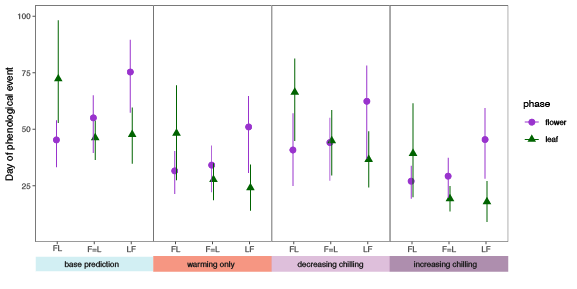
\includegraphics[width=\textwidth]{..//Plots/Flobuds_manuscript_figs/postergroups.png}
 %\caption{Alternative Fig. \ref{fig:preddy}.}
 %\end{figure}

\section*{Figures}
\begin{figure}[h!]
    \centering
         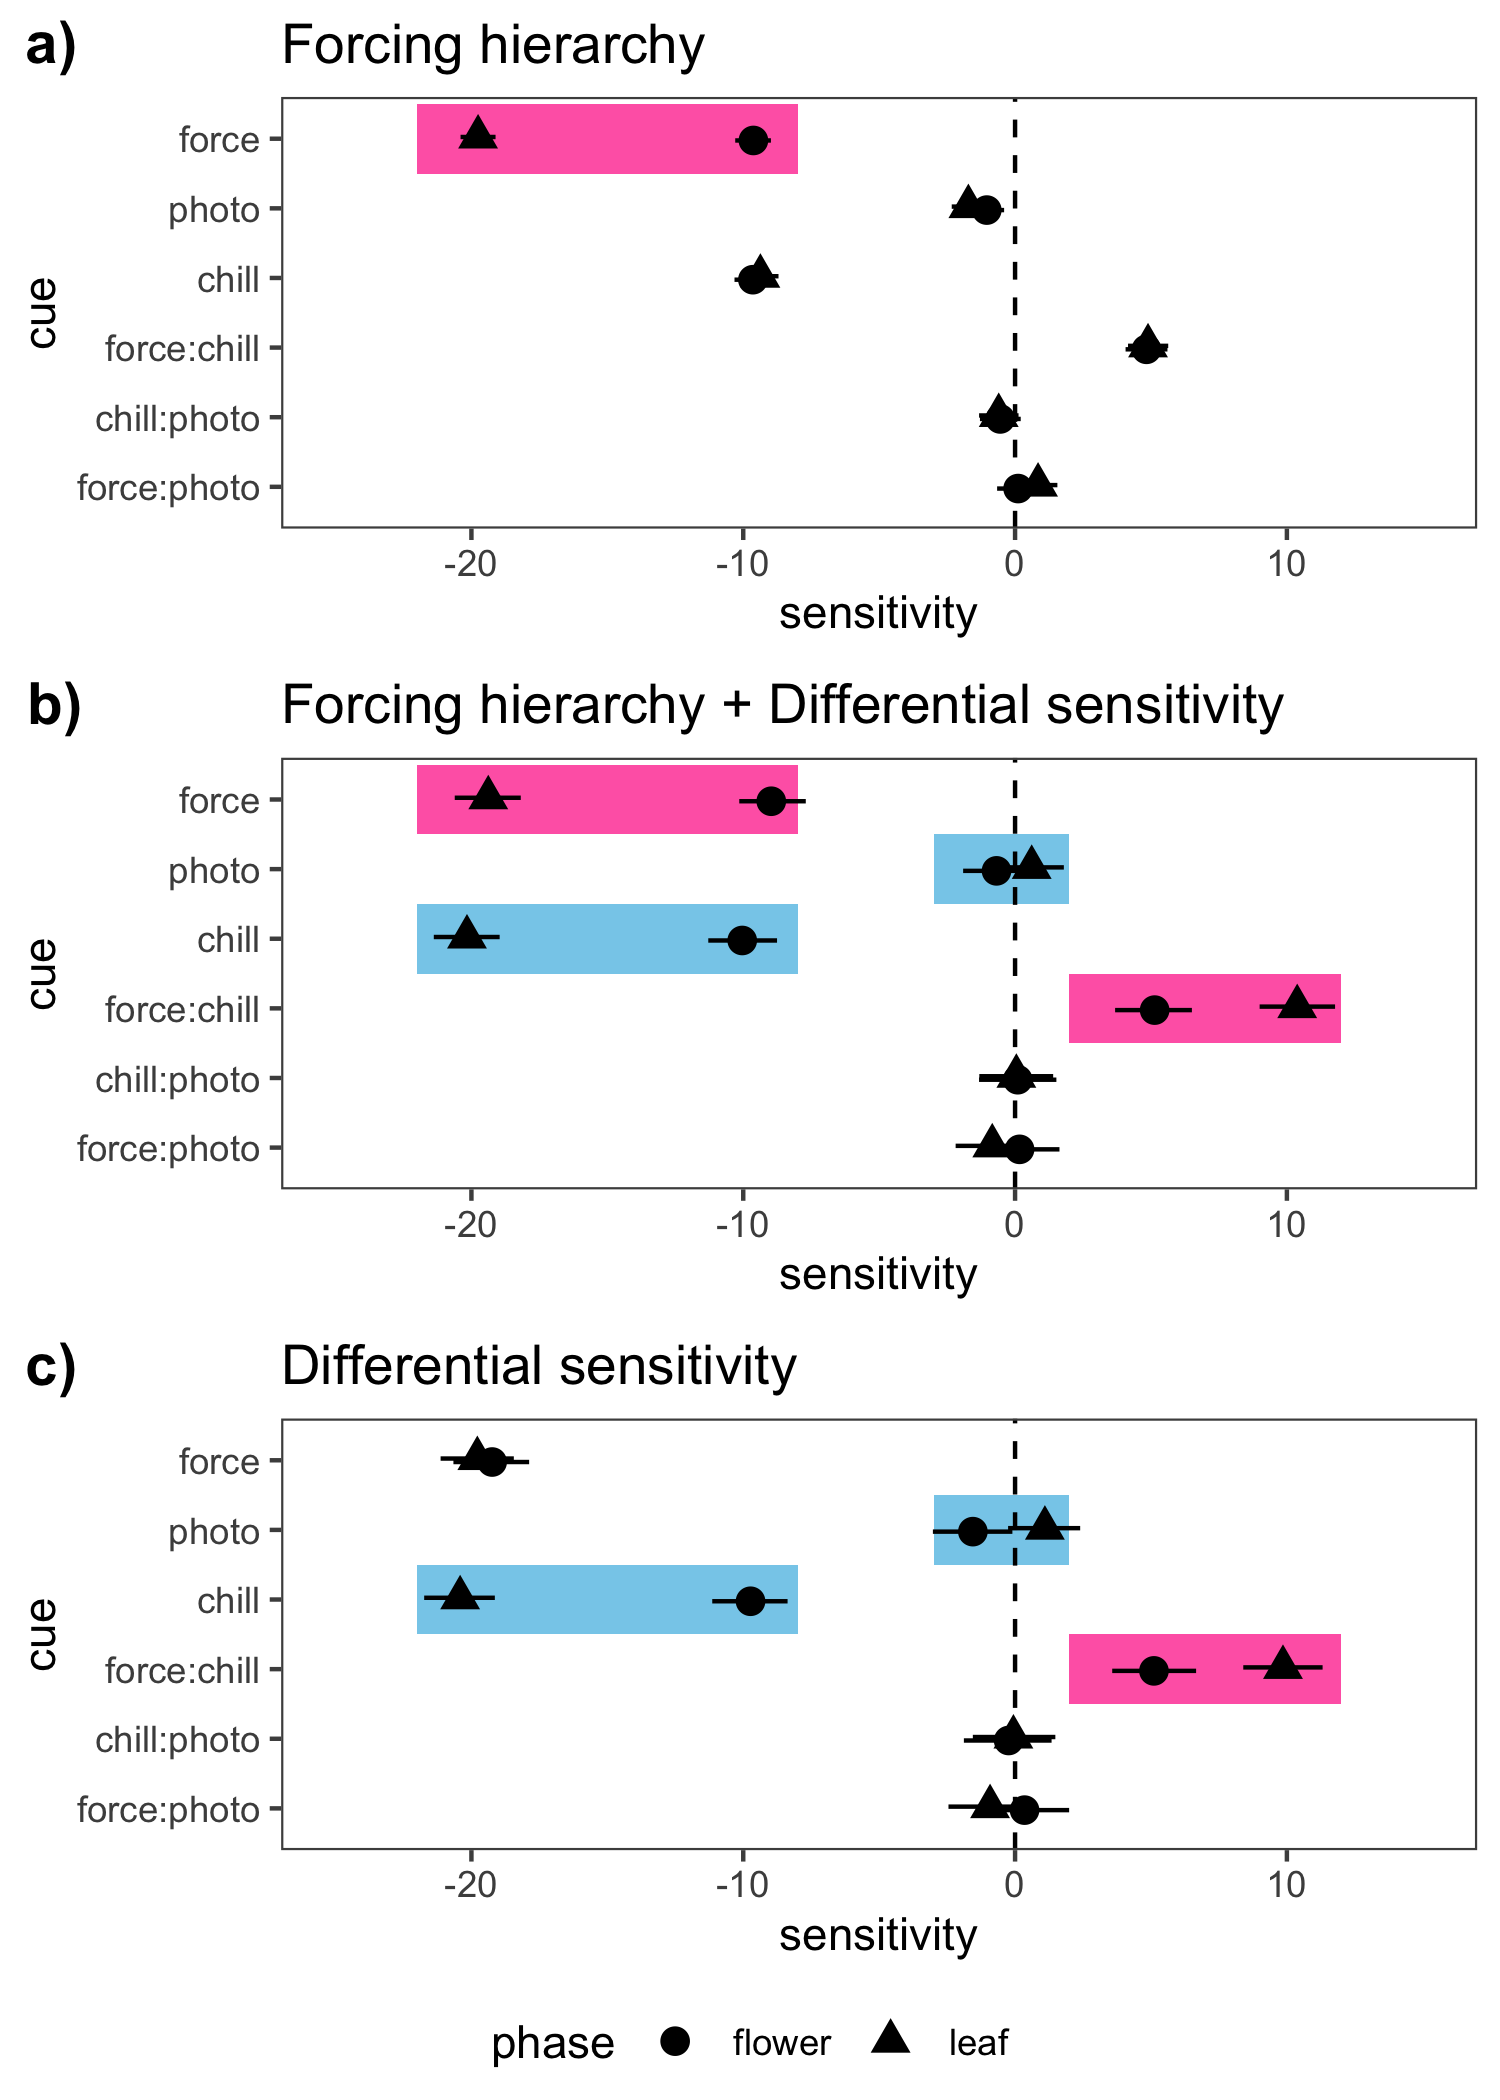
\includegraphics[width=.7\textwidth]{..//Plots/Flobuds_manuscript_figs/simulations.png}
    \caption{Characteristic sensitivity ($\Delta$ day of phenological event/ $\Delta$ environmental cue) patterns of the phenological response to changing cue levels for the two major flower-leaf sequence hypotheses.  \textbf{a)} displays a signature pattern of the forcing hierarchy hypothesis (FHH, pink boxes)---with the second phenophase in the sequence (in this case leafing) having a higher sensitivity to forcing than the first. \textbf{b)} depicts a scenario where both the FHH and the differential sensitivity hypothesis (DSH) contribute to flower-leaf sequence variation. Here the characteristic forcing sensitivity of the FHH is still apparent but the differential sensitivity to chilling and photoperiod is seen as well (blue boxes). \textbf{c)} highlights a typical sensitivity pattern produced by the DSH without the FHH. All plots above are based on simulations (see Supporting Information: Methods). Shapes indicate mean estimates and lines depict 95\% credible intervals from Bayesian hierarchical models with advances in phenology shown as negative numbers, and delays in phenology as positive numbers. } 
    \label{fig:simulations}
\end{figure}
\clearall % EMW5Dec20: Not sure if this will fix the float issue, but it might.

\begin{figure}[h!]
    \centering
         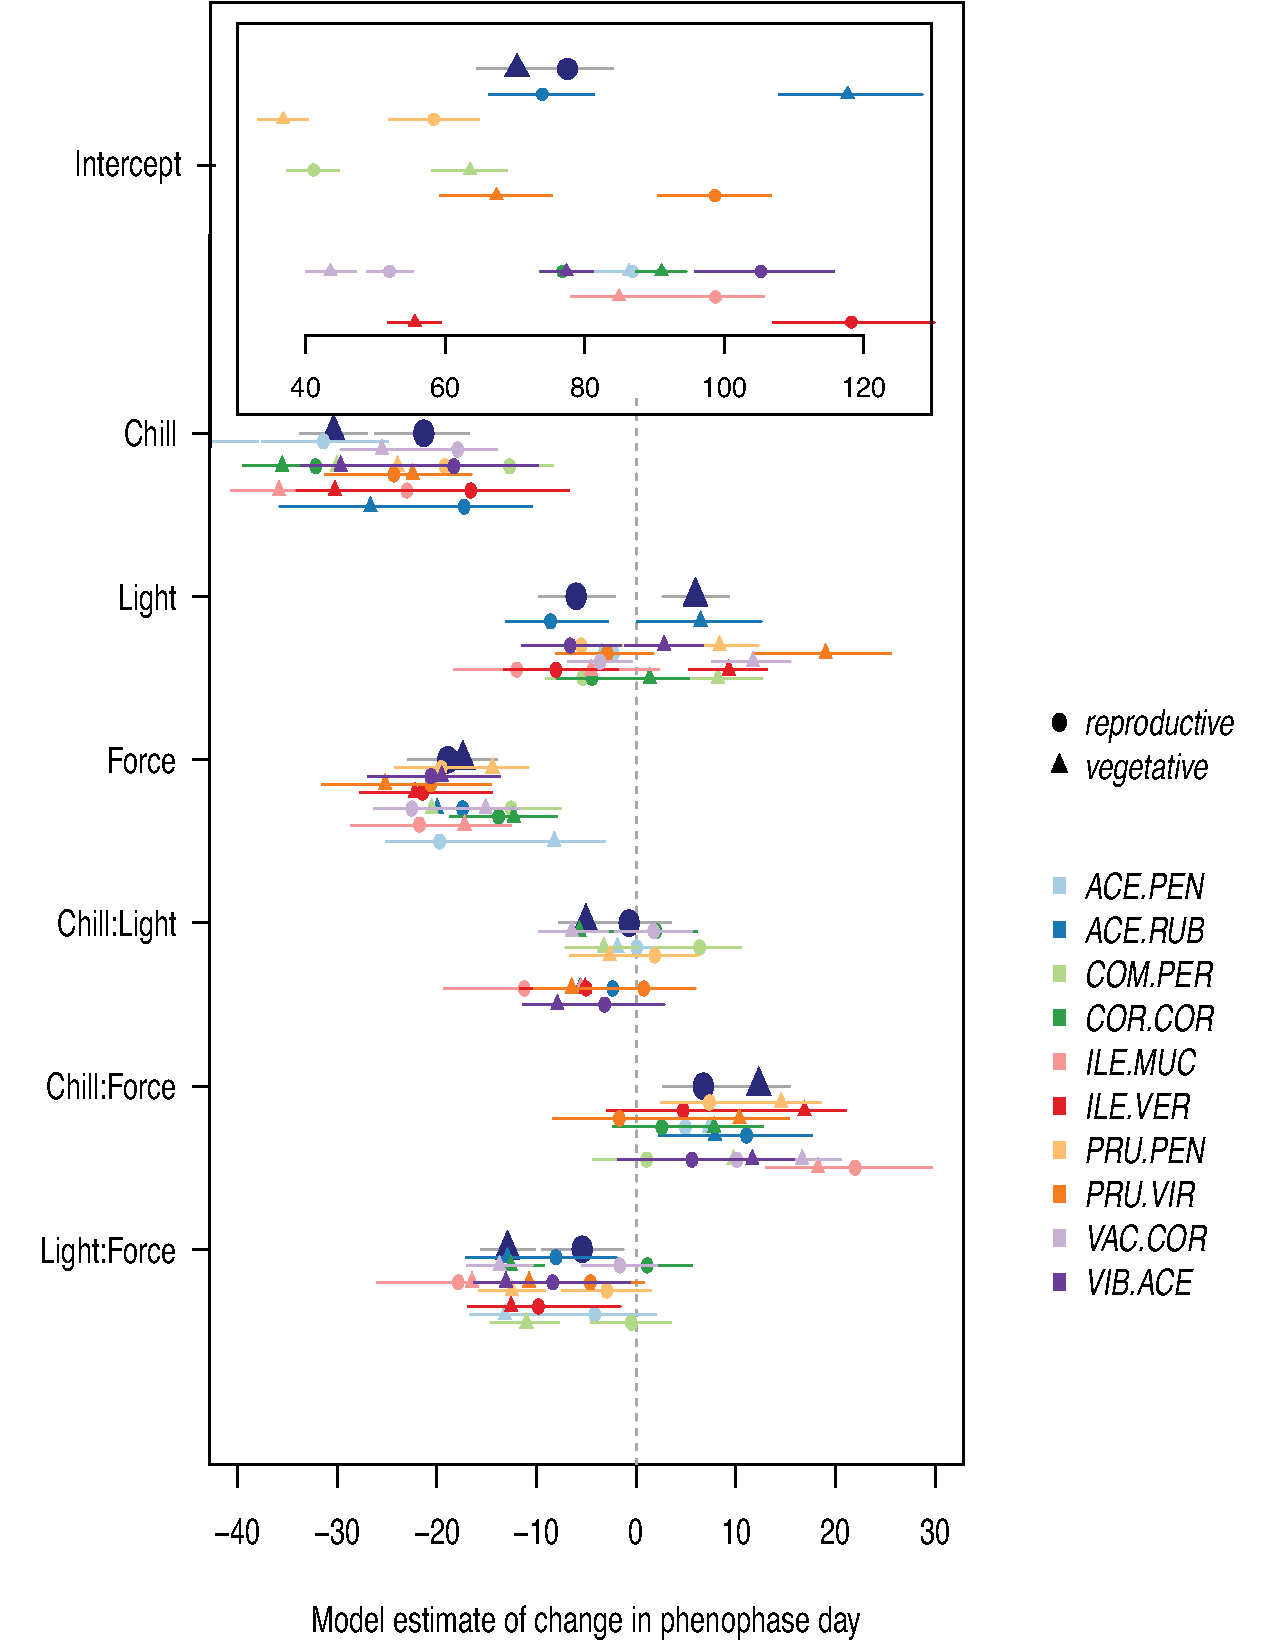
\includegraphics[width=0.9\textwidth]{..//Plots/Flobuds_manuscript_figs/budburstvsflowering.pdf}
         \caption{Effects of forcing temperature, chilling duration, and photoperiod on the leaf (circles) and flower (triangles) phenology of 10 temperate woody plant species collected from Harvard Forest (Petersham, MA, USA). Shapes indicate mean estimates and lines depict 50\% credible intervals (See Tab. \ref{tab:modelests}, Tab. \ref{tab:modelests2} for other intervals) from Bayesian hierarchical models with advances in phenology shown as negative numbers, and delays in phenology as positive numbers. Flower and leaf phenology differs in sensitivity ($\Delta$ day of phenological event/ $\Delta$ environmental cue) to these environmental cues.}
   % \caption{\textbf{Experimental results suggest differential sensitivity to environmental cues between flower and leaf buds}. We used a growth chamber manipulation and Bayesian hierarchical models to evaluate the phenological sensitivity ($\Delta$ day of phenological event/ $\Delta$ environmental cue) of flower and leaf buds to varying forcing temperatures, photoperiods, and duration of chilling.   Vegetative buds (circles) were more sensitive to chilling and cue interactions. Flower buds (triangles) advanced with photoperiod increases under all treatment combinations but leaf phenology was delayed with increasing photoperiod when chilling and forcing levels were low. Points indicate mean estimates and lines represent the 50\% credible intervals. These differential sensitivities dictate how FLS patterns vary with changing environmental conditions.}
    \label{fig:model}
\end{figure}

\begin{figure}[h!]
    \centering
         \includegraphics[width=\textwidth]{..//Plots/Flobuds_manuscript_figs/PHH_plot.png} 
    \caption{Phenological sensitivity ($\Delta$ phenological event/ $\Delta$ C$\degree$) to forcing temperatures of leaf (circles) and flower (triangles) phenology from 10 temperate deciduous woody plants at long (12 hour) photoperiod and long chilling duration treatments (8 weeks at 4\degree C). Shapes indicate mean estimates and lines depict 50\% credible intervals (See Tab. \ref{tab:phh} for other intervals) from Bayesian hierarchical models with advances in phenology shown as negative numbers. When photoperiod and chilling are high, most species follows the predicted pattern of the forcing hierarchy hypothesis (FHH), with the second phenophase of the sequence consistently more sensitive to forcing than the first. This result suggests that the FHH should be considered a special case of the differential sensitivity hypothesis (DSH) that occurs when the chilling and photoperiod requirements are met for both tissue types.}
    %\caption{\textbf{Under adequately long chilling duration and photoperiods, the phenological sensitivity ($\Delta$ phenological event/ $\Delta$ C$\degree$) follows the predicted pattern of the forcing hierarchy hypothesis (FHH), with the second phenophase of the sequence consistantly sensitive to forcing as the first.} After performing a growth chamber manipulation evaluate the phenological sensitivity of flower and leaf buds to varying level forcing temperatures, photoperiods, and duration of chilling, we subset out data to include only observation at high chilling and photoperiod levels. Using Bayesian hierarchical models, we quantified the differences in sensitivity to forcing for all species in our study. Points indicate mean estimates and lines depict 50\% credible intervals. Our finding indications that the FHH should be considered a special case of the differential sensitivity hypothesis (DSH) that occurs when the chilling and photoperiod requirements are well met for both bud types.} %emwhalloween20: I think here "Our finding indications that the FHH should be considered a special case of the differential sensitivity hypothesis (DSH) that occurs when the chilling and photoperiod requirements are well met for both bud types." works (though some journals are picky about no conclusions in figure captions, but I like it). 
    \label{fig:FHH}
\end{figure}

\pagebreak

\begin{figure}[h!]
    \centering
 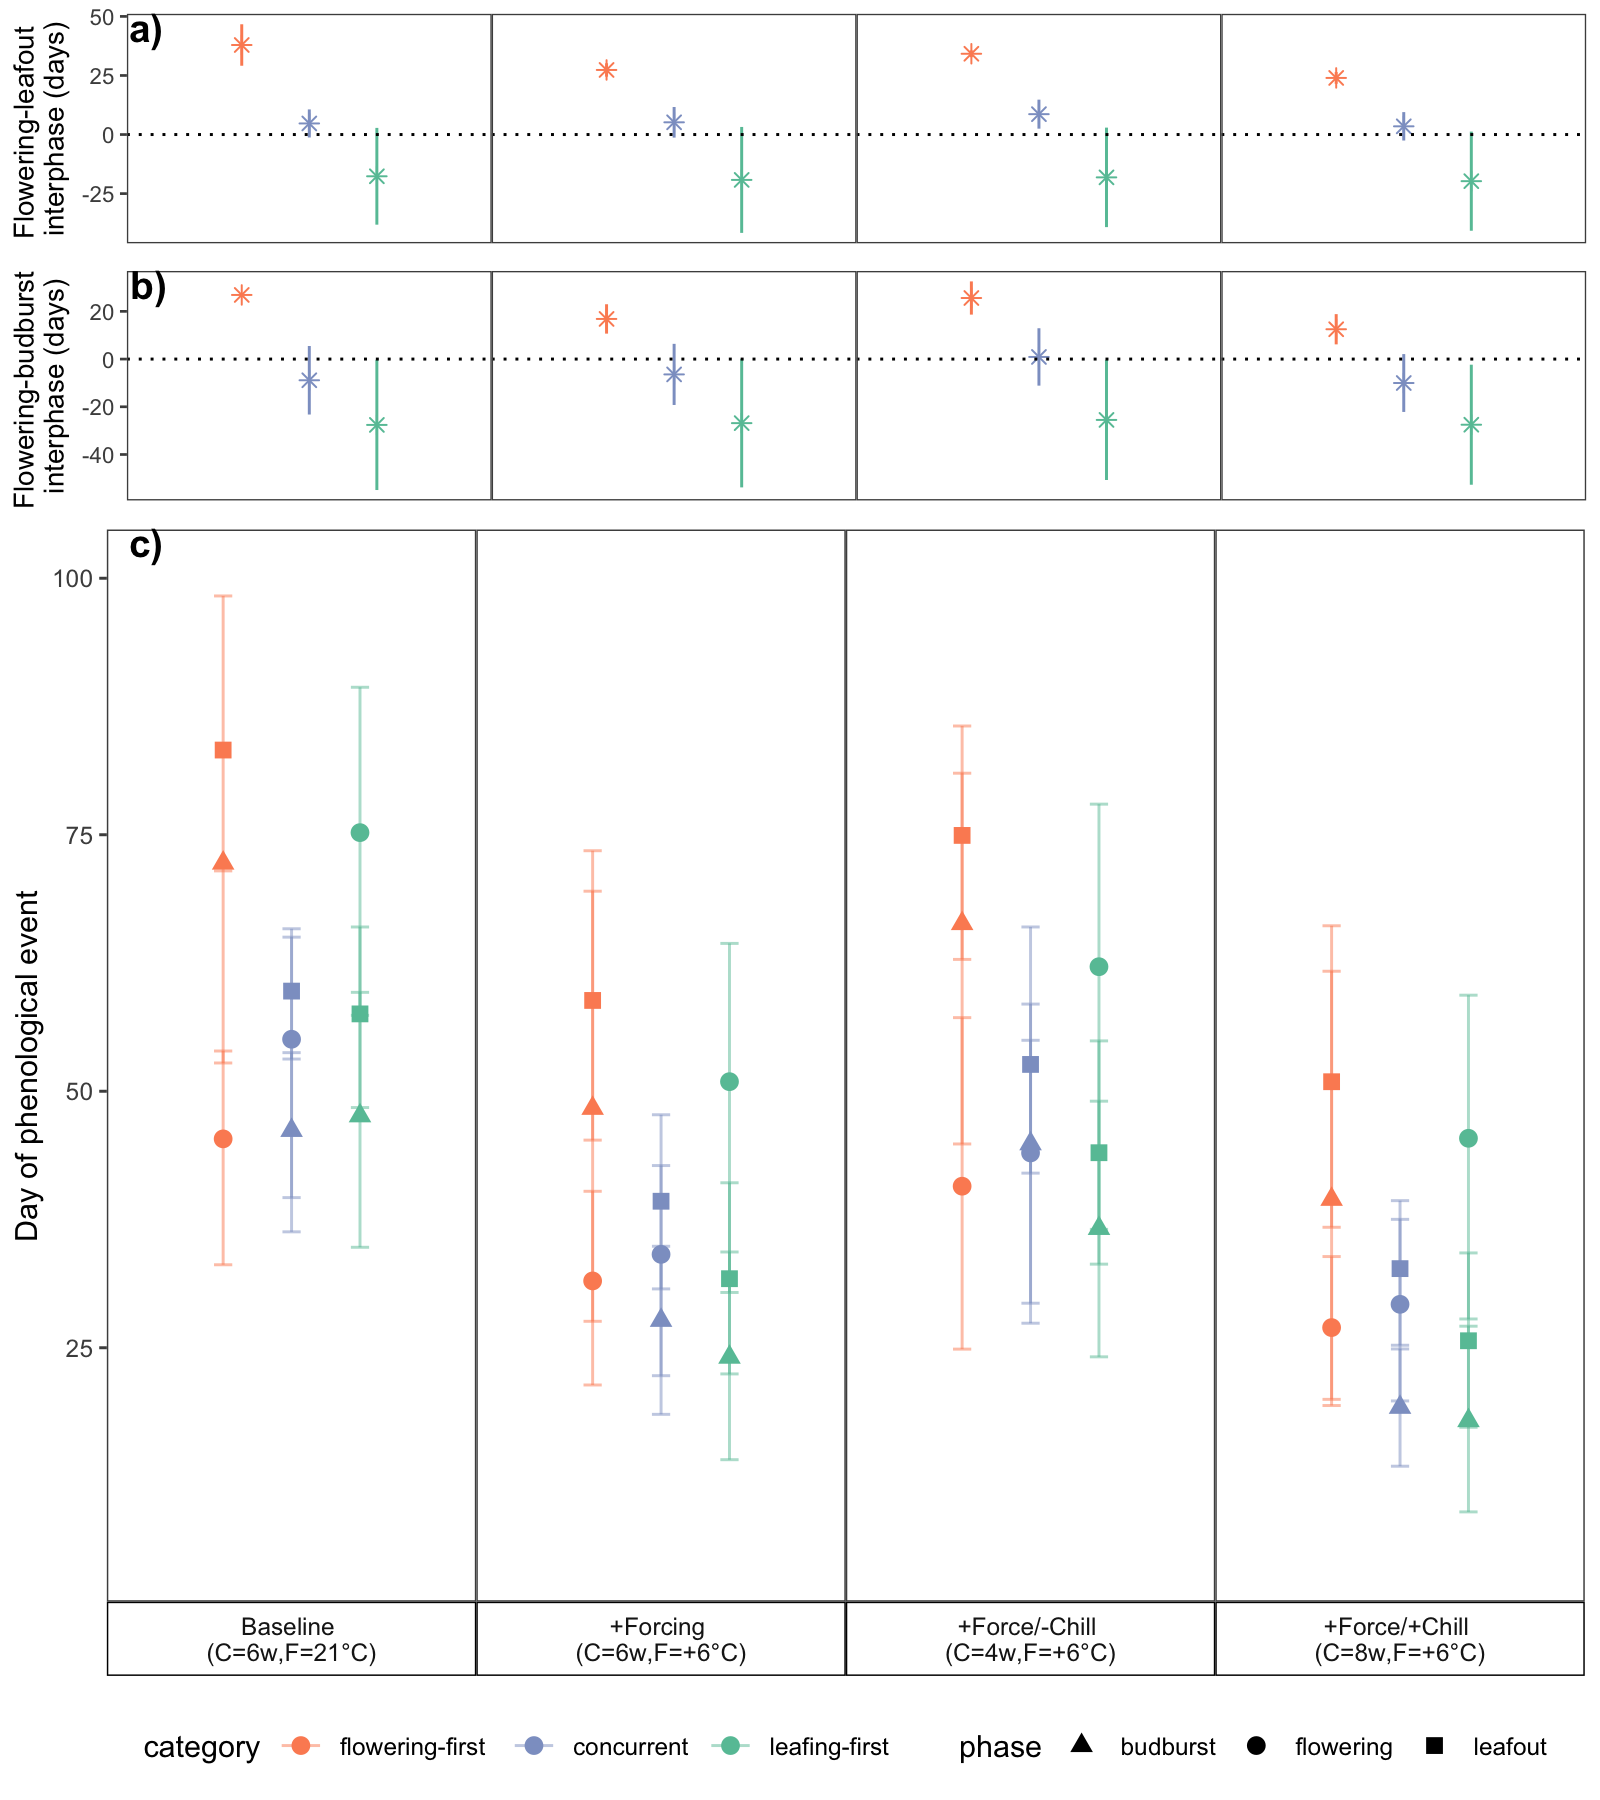
\includegraphics[width=\textwidth]{..//Plots/Flobuds_manuscript_figs/posteriorgroups_go.png} 
    \caption{Projected shifts in flower-leaf sequences under current environmental conditions (base prediction) and three climate change scenarios predict that FLS differ among the three major FLS types and will be strongest is flowering-first species. Predictions are based on species-level posterior estimates grouped by FLS category (flowering-first, concurrent, leafing-first) from Bayesian hierarchical models comparing flower (circles) and leaf (triangles) phenological responses to variable chilling duration and forcing temperatures. Shapes represent the mean estimates and lines represent the 50\% credible intervals. }
    %\caption{\textbf{Flower-leaf sequences (FLSs) of temperate, woody species will shift with climate change, but the magnitudes of these shifts vary by among FLS categories and depend on the specific dynamics of temperature at a given location.} We used Bayesian, hierarchical models comparing flower and leaf bud responses to variable temperature combinations to predict FLSs patterns under current climate conditions and three climate change scenarios;  an increase in spring warming alone (warm 5), increase in spring warming and increase in winter chilling (warm 5 +chill) and an increase in spring warming and decrease in winter chill (warm 5 -chill). We grouped the species-level posterior estimates by FLS category (flowering-first, concurrent, leafing-first). The points represent the mean estimates and the lines lines represent the 50\% credible intervals. In our study, all flowering-first species are wind-pollinated, and projected FLS shifts are most pronounced in some of these wind-pollinated, flowering-first shrubs. However, FLS shifts for all species depend on the relationship between forcing and chilling changes which is likely to vary by location with climate change.} %emwhalloween20: I like the figure, but need to re-write the caption to highlight species-group differences. 
    \label{fig:preddy}
\end{figure}



\end{document}
